\documentclass[xcolor=table,dvipsnames,table]{beamer}
\mode<presentation>
\usetheme{boxes}
\setbeamertemplate{navigation symbols}{}
% http://www.latex-community.org/forum/viewtopic.php?f=4&t=6694
\setbeamertemplate{navigation symbols}{\raisebox{5pt}{\makebox[\paperwidth]{\hfill\makebox[10pt]{\scriptsize\insertframenumber\vspace{1ex}}}}}
%\setbeamertemplate{footline}[frame number]
\setbeamertemplate{blocks}[shadow=false]
%\setbeamercolor*{block title}{fg=structure,bg=RoyalBlue!10}
\setbeamercolor*{block title example}{fg=structure,bg=RoyalBlue!10}
%\setbeamercolor*{block title example}{fg=BrickRed,bg=Goldenrod!10}
\setbeamercolor*{block title alerted}{fg=white,bg=black}
\addtobeamertemplate{block begin}{\pgfsetfillopacity{0.8}}{\pgfsetfillopacity{1}}
%\rowcolors{0}{RoyalBlue!20}{RoyalBlue!5}
\setbeamertemplate{caption}{\raggedright\insertcaption\par}

%\DeclareGraphicsRule{*}{mps}{*}{}

\usepackage{latexsym}
\usepackage{hyperref}
\usepackage{tikz}
\usetikzlibrary{calc,shapes,arrows,shadows,shapes.callouts,shapes.arrows,chains,positioning,trees}
\usepackage{solution}
\usepackage{calc}
\usepackage{pifont}
\usepackage{algorithmic}
\usepackage{pdfcomment}
\usepackage{color}

\newcommand{\cmark}{\ding{51}}
\newcommand{\xmark}{\ding{55}}

\newcommand{\highlight}[1]{{\color{blue}{#1}}}
\newcommand{\mycite}[1]{{\color{darkgray}{\footnotesize [#1]}}}

\DeclareMathOperator*{\argmin}{arg\,min}
\DeclareMathOperator*{\argmax}{arg\,max}
\DeclareMathOperator{\sign}{sign}
\DeclareMathOperator{\cnt}{Count}

\newcounter{mycallout}

\newcommand{\callouts}[3]{%
  \stepcounter{mycallout}
  \tikz[remember picture,baseline]{\node[anchor=base,inner sep=0,outer sep=0]%
    (\themycallout) {\colorbox{#1!20}{#3}};\pause\node[overlay,rectangle callout,%
    callout relative pointer={(0cm,0.5cm)},fill=#1!20] at ($(\themycallout.south)+(-0cm,-0.7cm)$){#2};}%
    }%

\raggedright

\newcount\lecturecount
\lecturecount=0
\AtBeginLecture{%
    \advance\lecturecount by 1
    \date{}
    \begin{frame}
    \begin{center}
    \titlepage
    \ifnum\lecturecount=1
    Part \the\lecturecount: \insertlecture
    \else
    Part \the\lecturecount: \insertlecture
    \fi
    \end{center}
    \end{frame}
}

\addtobeamertemplate{block begin}{\setlength\abovedisplayskip{0pt}}

%\newcommand{\example}[1]{{\color{BrickRed!50}{#1}}}
\newcommand{\maths}[1]{{\color{RoyalBlue!50}{#1}}}
\newcommand{\reference}[1]{{\color{RoyalBlue!30}\tiny [from #1]}}
\newcommand{\koehnref}{\reference{\href{http://www.statmt.org/book}{P.Koehn SMT book slides}}}


\begin{document}

\title{\color{MidnightBlue}Natural Language Processing}

\author{Anoop Sarkar \\ {\color{RoyalBlue!70}{\href{http://anoopsarkar.github.io/nlp-class}{anoopsarkar.github.io/nlp-class}}}}
\institute{\color{BrickRed}Simon Fraser University}
%\date{}
     
{
\addtocounter{framenumber}{-1}
\begin{frame}
\begin{center}
\vspace{8mm}

\includegraphics[scale=0.35]{figures/natlang-cky-logo}
\end{center}
\titlepage
\end{frame}
}



\lecture{Long distance dependencies}{}
\section{Long distance dependencies}

\begin{frame}
\frametitle{Long distance dependencies}
\begin{block}{Example}
\begin{itemize}[<+->]
\item {\color{blue} He} doesn't have very much confidence in {\color{blue} himself}
\item {\color{blue} She} doesn't have very much confidence in {\color{blue} herself}
\end{itemize}

\pause
\end{block}
\begin{block}{n-gram Language Models: $P(w_i \mid w_{i-n+1}^{i-1})$}
\begin{eqnarray*}
P(\text{himself} &\mid& \text{confidence}, \text{in} ) \\
P(\text{herself} &\mid& \text{confidence}, \text{in} ) 
\end{eqnarray*}
\end{block}

\pause
\begin{block}{What we want: $P(w_i \mid w_{<i})$}
\begin{eqnarray*}
P(\text{himself} &\mid& \text{He}, \ldots, \text{confidence} ) \\
P(\text{herself} &\mid& \text{She}, \ldots, \text{confidence} ) 
\end{eqnarray*}
\end{block}
\end{frame}

\begin{frame}{Long distance dependencies}
\framesubtitle{Other examples}	
\begin{itemize}[<+->]
	\item \textbf{Selectional preferences}: \textit{I ate lunch with a {\color{blue} fork}} vs.\ \textit{I ate lunch with a {\color{blue} backpack}}
	\item \textbf{Topic}: \textit{Babe Ruth was able to touch the home {\color{blue} plate} yet again} vs.\ \textit{Lucy was able to touch the home {\color{blue} audiences} with her humour}
	\item \textbf{Register}: Consistency of register in the entire sentence, e.g.\ informal (Twitter) vs.\ formal (scientific articles)
\end{itemize}
\end{frame}

\begin{frame}
\frametitle{Language Models}
\begin{block}{Chain Rule and ignore some history: the trigram model}
\begin{eqnarray*}
\lefteqn{p(w_1, \ldots, w_n) } \\
&\approx& p(w_1) p(w_2 \mid w_1) p(w_3 \mid w_1, w_2) \ldots p(w_n \mid w_{n-2}, w_{n-1}) \\
&\approx& \prod_{t} p(w_{t+1} \mid w_{t-1}, w_t)
\end{eqnarray*}
\end{block}
\pause
\begin{block}{How can we address the long-distance issues?}
\begin{itemize}
\item Skip $n$-gram models. Skip an arbitrary distance for $n$-gram context.
\item Variable $n$ in $n$-gram models that is adaptive
\item {\bf Problems}: Still "all or nothing". Categorical rather than soft.
\end{itemize}
\end{block}
\end{frame}

\lecture{Neural Language Models}{}

\begin{frame}
\frametitle{Neural Language Models}
\begin{block}{Use Chain rule and approximate using a neural network}
\[ p(w_1, \ldots, w_n) \approx \prod_{t} p(w_{t+1} \mid \underbrace{\phi(w_1, \ldots, w_t)}_{\text{capture history with vector $s(t)$}}) \]
\end{block}
\pause
\begin{block}{Recurrent Neural Network}
\begin{itemize}[<+->]
	\item Let $y$ be the output $w_{t+1}$ for current word $w_t$ and history $w_1, \ldots, w_t$
	\item $s(t) = f(U_{xh} \cdot w(t) + W_{hh} \cdot s(t-1))$ where $f$ is a sigmoid
	\item $s(t)$ encapsulates history using single vector of size $h$
	\item Output word at time step $w_{t+1}$ is provided by $y(t)$
	\item $y(t) = g(V_{hy} \cdot s(t))$ where $g$ is softmax
\end{itemize}
\end{block}
\end{frame}

\begin{frame}{Neural Language Models}
\framesubtitle{Recurrent Neural Network}
\begin{columns}
\begin{column}{0.4\textwidth}
\begin{block}{Single time step in RNN:}
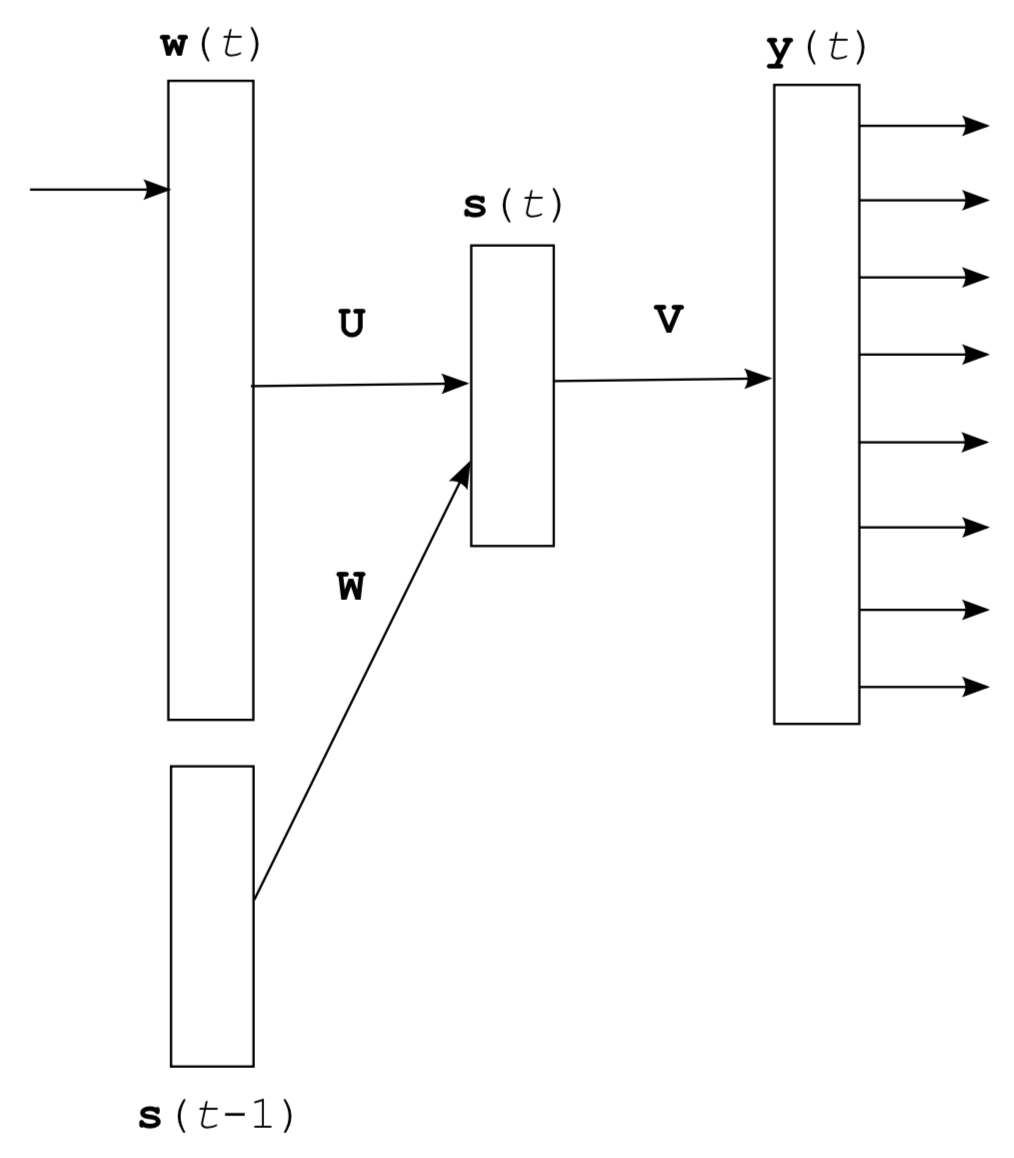
\includegraphics[scale=0.3]{figures/nlm/mikolovrnn.png}
\end{block}
\end{column}
\begin{column}{0.6\textwidth}
{\small
\begin{itemize}[<+->]
	\item Input layer is a one hot vector and output layer $\mathbf{y}$ have the same dimensionality as vocabulary (10K-200K). 
	\item One hot vector is used to look up word embedding $\mathbf{w}$
	\item ``Hidden'' layer $\mathbf{s}$ is orders of magnitude smaller (50-1K neurons)
	\item $U$ is the matrix of weights between input and hidden layer
	\item $V$ is the matrix of weights between hidden and output layer
	\item Without recurrent weights $W$, this is equivalent to a bigram feedforward language model
\end{itemize}
}
\end{column}
\end{columns}
\end{frame}

\begin{frame}{Neural Language Models}
\framesubtitle{Recurrent Neural Network}
\begin{figure}[t]
\centering
\begin{tikzpicture}[->,thick]
\scriptsize
\tikzstyle{main}=[minimum size = 7mm, thick, draw =black!80, node distance = 12mm]
\foreach \name in {1,...,6}
    \node[main, fill = yellow!80] (y\name) at (\name*2,1.5) {$\mathbf{y}(\name )$};
\foreach \name in {1,...,6}
    \node[main, fill = blue!20] (h\name) at (\name*2,0) {$\mathbf{s}(\name )$};
\foreach \name in {1,...,6}
    \node[main] (x\name) at (\name*2,-1.5) {$\mathbf{w}(\name )$};
\foreach \h in {1,...,6}
       {
        \path (x\h) edge[left] node{$U_{xh}$} (h\h);
        \path (h\h) edge[left] node{$V_{hy}$} (y\h);
       }
\foreach \current/\next in {1/2,2/3,3/4,4/5,5/6} 
       {
        \path (h\current) edge[above] node{$W_{hh}$} (h\next);
       }
    %\node[main] (G-\name) at (\x,0) {$\name$};
\end{tikzpicture}
\end{figure}
\begin{block}{What is stored and what is computed:}
\begin{itemize}[<+->]
	\item Model parameters: $\mathbf{w} \in \mathbb{R}^x$ (word embeddings); $U_{xh} \in \mathbb{R}^{x \times h}; W_{hh} \in \mathbb{R}^{h \times h}; V_{hy} \in \mathbb{R}^{h \times y}$ where $y = |{\cal V}|$. 
	\item Vectors computed during forward pass: $\mathbf{s}(t) \in \mathbb{R}^h; \mathbf{y}(t) \in \mathbb{R}^y$ and each $\mathbf{y}(t)$ is a probability over vocabulary ${\cal V}$.
\end{itemize}
\end{block}
\end{frame}

\lecture{Training RNN Language Models}{}

\section{Training RNNs}

\begin{frame}{Neural Language Models}
\framesubtitle{Recurrent Neural Network}
\begin{block}{Computational Graph for an RNN Language Model}
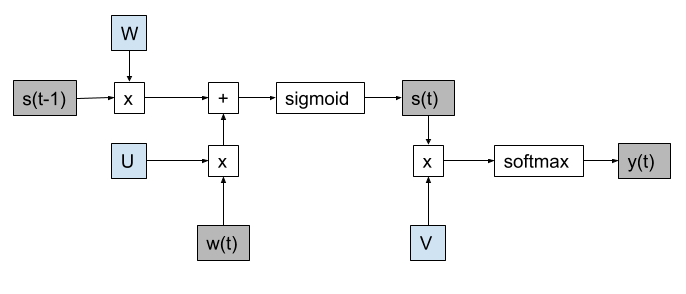
\includegraphics[width=\textwidth]{figures/nlm/mikolovrnn-graph.png}
\end{block}
\end{frame}

\begin{frame}{Training of RNNLM}
\begin{itemize}[<+->]
	\item The training is performed using Stochastic Gradient Descent (SGD)
	\item We go through all the training data iteratively, and update the weight matrices $U$, $W$ and $V$ (after processing every word)
	\item Training is performed in several ``epochs'' (usually 5-10)
	\item An epoch is one pass through the training data
\end{itemize}
\end{frame}

\begin{frame}{Training of RNNLM}
\begin{itemize}[<+->]
	\item Gradient of the error vector in the output layer $\mathbf{e}_o(t)$ is computed using a cross entropy criterion:
	\[ \mathbf{e}_o(t) = \mathbf{d}(t) - \mathbf{y}(t) \]
	\item $\mathbf{d}(t)$ is a target vector that represents the word $w(t+1)$ represented as a one-hot (1-of-${\cal V}$) vector
\end{itemize}
\end{frame}

\begin{frame}{Training of RNNLM}
\begin{itemize}[<+->]
	\item Weights $V$ between the hidden layer $s(t)$ and the output layer $y(t)$ are updated as
	\[ V^{(t+1)} = V^{(t)} + \mathbf{s}(t) \cdot \mathbf{e}_o(t) \cdot \alpha \]
	\item where $\alpha$ is the learning rate
\end{itemize}
\end{frame}

\begin{frame}{Training of RNNLM}
\begin{itemize}[<+->]
	\item Next, gradients of errors are propagated from the output layer to the hidden layer
	\[ \mathbf{e}_h(t) = d_h(\mathbf{e}_o \cdot V, t) \]
	\item where the error vector is obtained using function $d_h()$ that is applied element-wise:
	\[ d_{hj} = x \cdot s_j(t) (1 - s_j(t))\]
\end{itemize}
\end{frame}

\begin{frame}{Training of RNNLM}
\begin{itemize}[<+->]
	\item Weights $U$ between the input layer $w(t)$ and the hidden layer $s(t)$ are then updated as
	\[ U^{(t+1)} = U^{(t)} + \mathbf{w}(t) \cdot \mathbf{e}_h(t) \cdot \alpha \]
	\item Similarly the word embeddings $\mathbf{w}$ can also be updated using the error gradient.
\end{itemize}
\end{frame}

\begin{frame}{Training of RNNLM: Backpropagation through time}
\begin{itemize}[<+->]
	\item The recurrent weights $W$ are updated by unfolding them in time and training the network as a deep feedforward neural network.
	\item The process of propagating errors back through the recurrent weights is called Backpropagation Through Time (BPTT).
\end{itemize}
\end{frame}

\begin{frame}{Training of RNNLM: Backpropagation through time}
\framesubtitle{Fig.\ from \cite{Mikolov2010}: RNN unfolded as a deep feedforward network 3 time steps back in time}
\centering
\begin{figure}
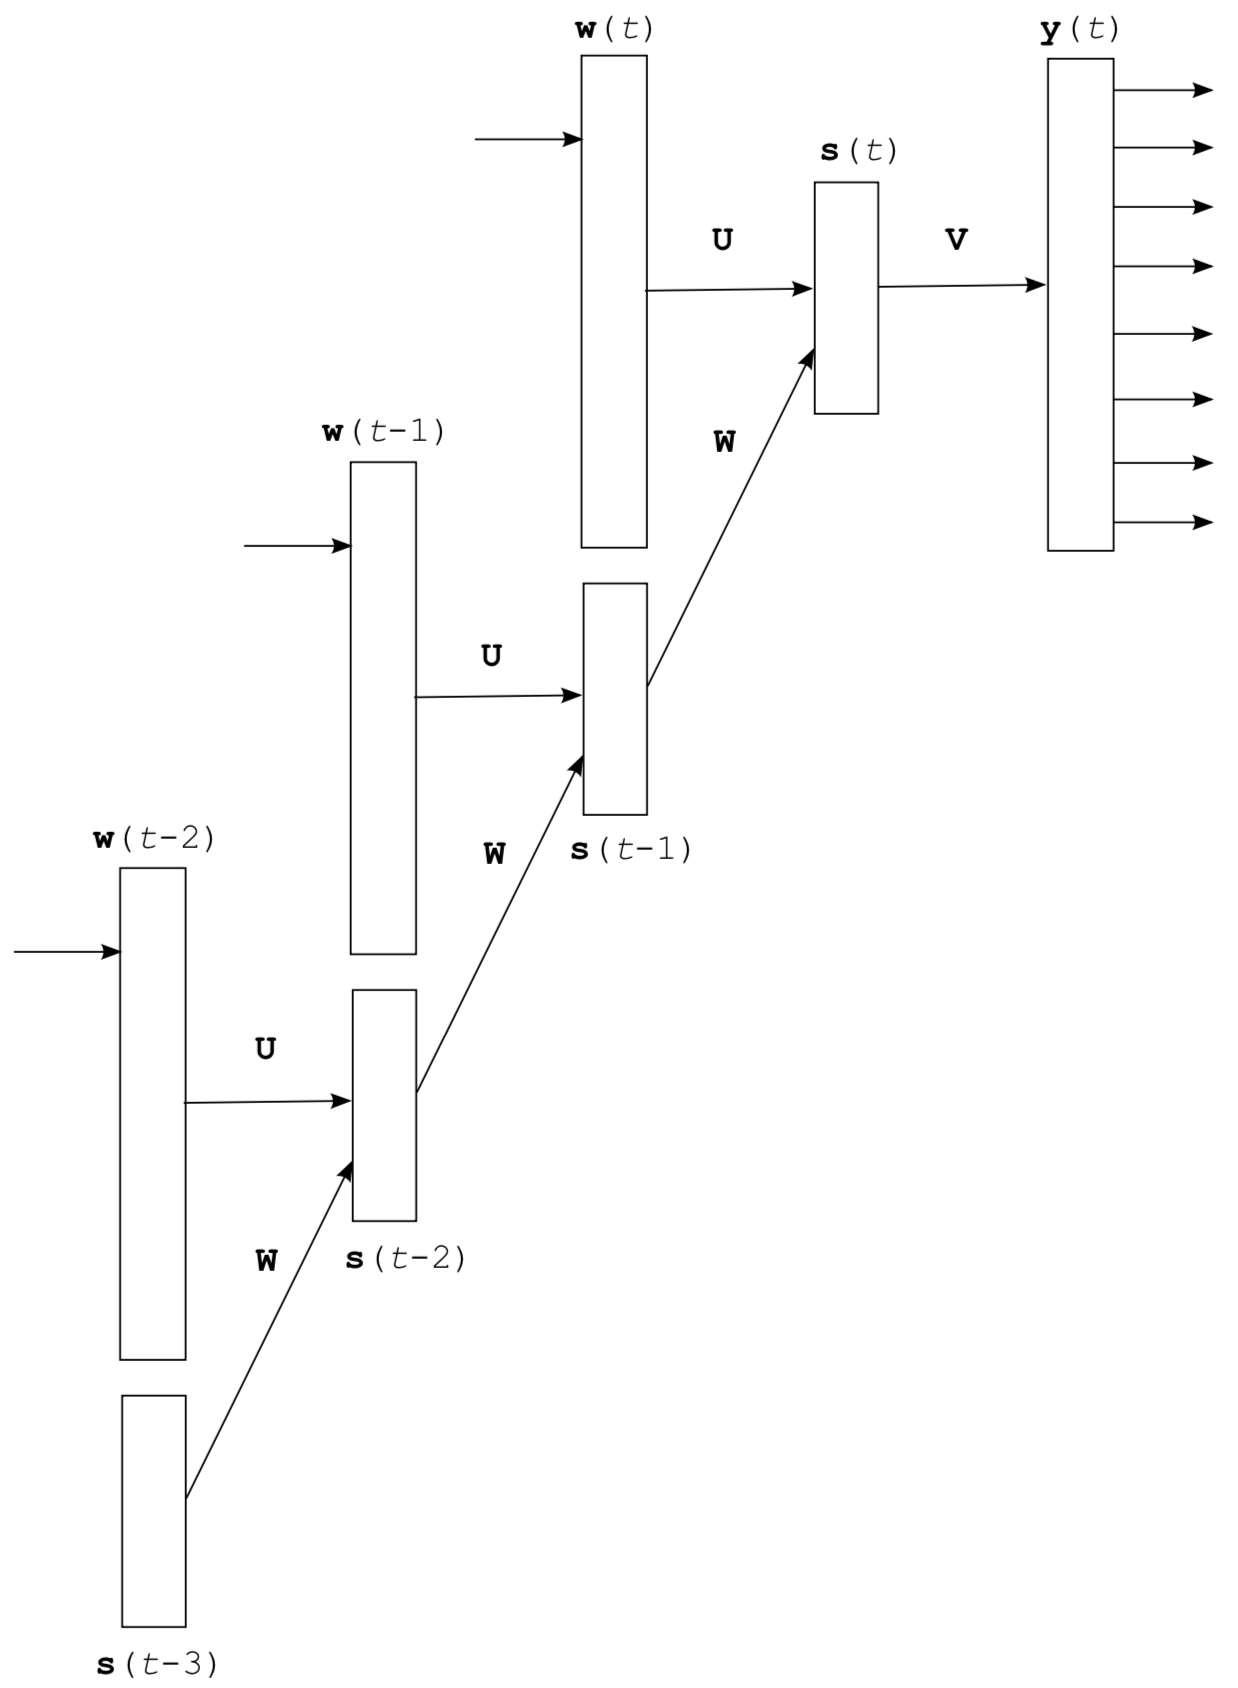
\includegraphics[scale=0.25]{figures/nlm/rnn-bptt.png}
\end{figure}
\end{frame}

\begin{frame}{Training of RNNLM: Backpropagation through time}
\begin{itemize}[<+->]
	\item Error propagation is done recursively as follows (it requires the states of the hidden layer from the previous time steps $\tau$ to be stored):
	\[ \mathbf{e}(t - \tau - 1) = d_h(\mathbf{e}_h(t-\tau) \cdot W, t - \tau -1) \]
	\item The error gradients quickly vanish as they get backpropagated in time (in rare cases the errors can explode)
	\item We use gated RNNs to stop gradients from vanishing or exploding. 
	\item Popular gated RNNs are \textit{long short-term memory} RNNs aka LSTMs and \textit{gated recurrent units} aka GRUs. 
\end{itemize}
\end{frame}

\begin{frame}{Training of RNNLM: Backpropagation through time}
\begin{itemize}[<+->]
	\item The recurrent weights $W$ are updated as:
	\[ W^{(t+1)} = W^{(t)} + \sum_{z=0}^T \mathbf{s}(t - z - 1) \cdot \mathbf{e}_h(t-z) \cdot \alpha \]
	\item Note that the matrix $W$ is changed in one update at once, not during backpropagation of errors.
\end{itemize}

\end{frame}

\lecture{Sequence prediction using RNNs}{}
\newcommand{\postag}[1]{{\color{red}/#1}}
\newcommand{\nertag}[1]{{\color{blue}/#1}}

\section{Recurrent networks for sequence tagging}

\begin{frame}
\frametitle{Representation: finding the right parameters}
\begin{block}{Problem: Predict ?? using context, $P(?? \mid \texttt{context})$ }
Profits\postag{N} soared\postag{V} at\postag{P} Boeing\postag{??} Co. , easily topping forecasts on Wall Street , as their CEO Alan Mulally announced first quarter results .
\end{block}
\pause
\begin{block}{Representation: history}
\begin{itemize}
\item The input is a tuple: $(x_{[1:n]}, i)$ [ignoring $y_{-1}$ for now]
\item $x_{[1:n]}$ are the $n$ words in the input
\item $i$ is the index of the word being tagged
\item For example, for $x_4$ = Boeing
\item We can use an RNN to summarize the entire context at $i=4$
    \begin{itemize}
    \item $x_{[1:i-1]}$ = (Profits, soared, at)
    \item $x_{[i+1:n]}$ = (Co., easily, ..., results, .)
    \end{itemize}
\end{itemize}
\end{block}
\end{frame}

\begin{frame}
\frametitle{Locally normalized RNN taggers}
\begin{block}{Log-linear model over history, tag pair $(h,t)$}
\[ \log \Pr(y \mid h) = \textbf{w} \cdot \textbf{f}(h, y) - log \sum_{y'} \exp \left( \textbf{w} \cdot \textbf{f}(h, y') \right) \]
\centering
$\textbf{f}(h, y)$ is a vector of feature functions
\end{block}
\pause
\begin{block}{RNN for tagging}
\begin{itemize}
\item Replace $\textbf{f}(h, y)$ with RNN hidden state $s(t)$
\item Define the output logprob: $\log \Pr(y \mid h) = \log y(t)$
\item $y(t) = g(V \cdot s(t))$ where $g$ is softmax
\item In neural LMs the output $y \in {\cal V}$ (vocabulary)
\item In sequence tagging using RNNs the output $y \in {\cal T}$ (tagset)
\end{itemize}
\[ \log \Pr( y_{[1:n]} \mid x_{[1:n]} ) = \sum_{i=1}^n \log \Pr(y_i \mid h_i) \]
\end{block}
\end{frame}

\begin{frame}{Bidirectional RNNs}
\framesubtitle{Fig.\ from \cite{Brakel2015}}
\begin{figure}[t]
\centering
\begin{tikzpicture}[->,thick]
\scriptsize
\tikzstyle{main}=[minimum size = 7mm, thick, draw =black!80, node distance = 12mm]
\foreach \name in {1,...,6}
    \node[main, fill = blue!20] (i\name) at (\name*2,.8) {$\mathbf{s}^b(\name )$};
\foreach \name in {1,...,6}
    \node[main, fill = blue!20] (h\name) at (\name*2,0) {$\mathbf{s}^f(\name )$};
\foreach \name in {1,...,6}
    \node[main] (x\name) at (\name*2,-1.5) {$\mathbf{x}(\name )$};
\foreach \h in {1,...,6}
       {
        \path (x\h) edge [bend right] (i\h);
        \path (x\h) edge (h\h);
       }
\foreach \current/\next in {1/2,2/3,3/4,4/5,5/6} 
       {
        \path (i\next) edge (i\current);
        \path (h\current) edge (h\next);
       }
    %\node[main] (G-\name) at (\x,0) {$\name$};
\end{tikzpicture}
\caption{Bidirectional RNN}
\label{fig:birnn}
\end{figure}
\end{frame}

\begin{frame}{Bidirectional RNNs can be Stacked}
\framesubtitle{Fig.\ from \cite{Brakel2015}}
\begin{figure}[t]
\centering
\begin{tikzpicture}[->,thick]
\scriptsize
\tikzstyle{main}=[minimum size = 7mm, thick, draw =black!80, node distance = 12mm]
\foreach \name in {1,...,6}
    \node[main, fill = blue!20] (l\name) at (\name*2,2.3) {$\mathbf{s}^f_2(\name )$};
\foreach \name in {1,...,6}
    \node[main, fill = blue!20] (k\name) at (\name*2,3.1) {$\mathbf{s}^b_2(\name )$};
\foreach \name in {1,...,6}
    \node[main, fill = blue!20] (h\name) at (\name*2,0) {$\mathbf{s}^f_1(\name )$};
\foreach \name in {1,...,6}
    \node[main, fill = blue!20] (i\name) at (\name*2,.8) {$\mathbf{s}^b_1(\name )$};
\foreach \name in {1,...,6}
    \node[main] (x\name) at (\name*2,-1.5) {$\mathbf{x}(\name )$};
\foreach \h in {1,...,6}
       {
        \path (x\h) edge [bend left] (i\h);
        \path (x\h) edge (h\h);
        \path (i\h) edge [bend left] (k\h);
        \path (h\h) edge [bend right] (l\h);
%        \path (h\h) edge [bend left] (k\h);
%        \path (i\h) edge (l\h);
       }
\foreach \current/\next in {1/2,2/3,3/4,4/5,5/6} 
       {
        \path (i\next) edge (i\current);
        \path (h\current) edge (h\next);
        \path (k\next) edge (k\current);
        \path (l\current) edge (l\next);
       }
    %\node[main] (G-\name) at (\x,0) {$\name$};
\end{tikzpicture}
\caption{Two Bidirectional RNNs stacked on top of each
other}
\label{fig:birnn}
\end{figure}
\end{frame}

\lecture{Training RNNs on GPUs}{}

\section{RNNs In Practice}

\begin{frame}{Parallelizing RNN computations}
	\framesubtitle{Fig.\ from \cite{Brakel2015}}
    Apply RNNs to \emph{batches} of sequences\\
        Present the data as a 3D tensor of $(T \times B \times F)$.
        Each dynamic update will now be a matrix multiplication.
\begin{figure}
\centering
\resizebox{4cm}{2.5cm}{
\begin{tikzpicture}
\tikzset{every cell/.style={draw=white}}
\tikzset{every cell 1/.style={fill=gray}}

   \foreach \row [count=\y] in {%
     {1,1,1,1,1,1,1,1,1,1,1,1,1,1,1,1,1,1,1,1},%
     {1,1,1,1,1,1,1,1,1,1,1,1,1,1,1,1,1,1,0,0},%
     {1,1,1,1,1,1,1,1,1,1,1,1,1,1,1,0,0,0,0,0},%
     {1,1,1,1,1,1,1,1,1,1,1,1,1,1,1,1,1,0,0,0},%
     {1,1,1,1,1,1,1,1,1,1,1,1,1,1,1,1,1,0,0,0},%
     {1,1,1,1,1,1,1,1,1,1,1,1,1,1,1,1,0,0,0,0},%
     {1,1,1,1,1,1,1,1,1,1,1,1,1,1,1,1,1,1,0,0}}
     \foreach \cell [count=\x] in \row  {
        \path [every cell/.try, every cell \cell/.try]
        (\x,-\y) rectangle ++(1,1);
       }
\end{tikzpicture}
}
\end{figure}
\end{frame}

\begin{frame}{Binary Masks}
\framesubtitle{Fig.\ from \cite{Brakel2015}}
    A \emph{mask} matrix may be used to aid with computations that ignore the padded zeros.
\begin{figure}
\centering
\resizebox{\textwidth}{!}{
\begin{tikzpicture}
\tikzset{every cell/.style={draw=black}}
\tikzset{every cell 1/.style={draw=black}}

   \foreach \row [count=\y] in {%
     {1,1,1,1,1,1,1,1,1,1,1,1,1,1,1,1,1,1,1,1},%
     {1,1,1,1,1,1,1,1,1,1,1,1,1,1,1,1,1,1,0,0},%
     {1,1,1,1,1,1,1,1,1,1,1,1,1,1,1,0,0,0,0,0},%
     {1,1,1,1,1,1,1,1,1,1,1,1,1,1,1,1,1,0,0,0},%
     {1,1,1,1,1,1,1,1,1,1,1,1,1,1,1,1,1,0,0,0},%
     {1,1,1,1,1,1,1,1,1,1,1,1,1,1,1,1,0,0,0,0},%
     {1,1,1,1,1,1,1,1,1,1,1,1,1,1,1,1,1,1,0,0}}
     \foreach \cell [count=\x] in \row  {
        \path [every cell/.try, every cell \cell/.try]
        (\x,-\y) rectangle ++(1,1) node[below left] {$\cell$};
       }
\end{tikzpicture}
}
\end{figure}
\end{frame}

\begin{frame}{Binary Masks}
\framesubtitle{Fig.\ from \cite{Brakel2015}}
    It may be necessary to (partially) sort your data.
\begin{figure}
\centering
\resizebox{8cm}{5cm}{
\begin{tikzpicture}
\tikzset{every cell/.style={draw=black}}
\tikzset{every cell 1/.style={fill=gray}}

   \foreach \row [count=\y] in {%
     {1,1,0,0,0,0,0,0,0,0,0,0,0,0,0,0,0,0,0,0},%
     {1,1,1,1,1,1,1,1,1,1,1,1,1,1,1,1,1,1,1,1},%
     {1,1,1,0,0,0,0,0,0,0,0,0,0,0,0,0,0,0,0,0},%
     {1,1,1,1,1,0,0,0,0,0,0,0,0,0,0,0,0,0,0,0},%
     {1,1,1,1,1,1,0,0,0,0,0,0,0,0,0,0,0,0,0,0},%
     {1,1,1,1,0,0,0,0,0,0,0,0,0,0,0,0,0,0,0,0}}
     \foreach \cell [count=\x] in \row  {
        \path [every cell/.try, every cell \cell/.try]
        (\x,-\y) rectangle ++(1,1);
       }
\end{tikzpicture}
}
\end{figure}
\end{frame}

\begin{frame}
\setbeamertemplate{bibliography item}[text]
\begin{thebibliography}{10}


\bibitem{Mikolov2010}
\alert{Tomas Mikolov}
\newblock {Recurrent Neural Networks for Language Models. Google Talk.}
\newblock 2010.

\bibitem{Brakel2015}
\alert{Philemon Brakel}
\newblock {MLIA-IQIA Summer School notes on RNNs}
\newblock 2015.

\end{thebibliography}
\end{frame}



\section*{Acknowledgements}

\begin{frame}
\centering
\begin{alertblock}{Acknowledgements}
Many slides borrowed or inspired from lecture notes by Michael Collins, Chris Dyer, Kevin Knight, Philipp Koehn, Adam Lopez, Graham Neubig and Luke Zettlemoyer from their NLP course materials. 

\bigskip

All mistakes are my own.

\bigskip

A big thank you to all the students who read through these notes and helped me improve them.

\end{alertblock}
\end{frame}



\end{document}
